%----------------------------------------------------------------------------------------
%	PACKAGES AND OTHER DOCUMENT CONFIGURATIONS
%----------------------------------------------------------------------------------------

\documentclass{article}
\usepackage{array}
\usepackage[english]{babel}
\usepackage[letterpaper,top=2cm,bottom=2cm,left=3cm,right=3cm,marginparwidth=1.75cm]{geometry}
\usepackage{amsmath}
\usepackage{graphicx}
\usepackage{float}
\usepackage[colorlinks=true, allcolors=blue]{hyperref}
\usepackage{todonotes}
\graphicspath{ {resources/} }

\title{Heimdall - A Kubernetes Extension}
\author{Bryan Keane}

\begin{document}

\begin{titlepage}

    \newcommand{\HRule}{\rule{\linewidth}{0.5mm}} 
    \center
    
    
    %----------------------------------------------------------------------------------------
    %	LOGO SECTION
    %----------------------------------------------------------------------------------------
    \begin{center}
        
\includegraphics{setu_logo.png}
    \end{center}
     
    %----------------------------------------------------------------------------------------
    
     
    %----------------------------------------------------------------------------------------
    %	HEADING SECTIONS
    %----------------------------------------------------------------------------------------
    \textsc{\Large Bachelor of Science (Hons) Applied Computing}\\[0.25cm]
    
    
    %----------------------------------------------------------------------------------------
    %	TITLE SECTION
    %----------------------------------------------------------------------------------------
    
    \HRule \\[0.75cm]
    { \huge \bfseries Heimdall - A Kubernetes Extension}\\[0.3cm] %document
    \HRule \\[1.0cm]
     
    %----------------------------------------------------------------------------------------
    %	AUTHOR SECTION
    %----------------------------------------------------------------------------------------
    
    \begin{minipage}{0.4\textwidth}
    \begin{flushleft} \large
    \emph{Author:}\\
    Bryan Keane 
    \end{flushleft}
    \end{minipage}
    ~
    \begin{minipage}{0.4\textwidth}
    \begin{flushright} \large
    \emph{Supervisor:} \\
    Lucy White
    \end{flushright}
    \end{minipage}\\[2cm]
    
\end{titlepage}

\newpage

\tableofcontents
\newpage

\listoffigures
\newpage

\listoftables
\newpage



\section{Plagiarism Declaration}
I declare that this material, which I now submit for assessment, is entirely my own work and has not been taken from the work of others, save and to the extent that such work has been cited and acknowledged within the text of my work. I understand that plagiarism, collusion, and copying are grave and severe offences in the university and accept the penalties that would be imposed should I engage in plagiarism, collusion or copying. I have read and understood the Assignment Regulations. I have identified and included the source of all other facts, ideas, opinions, and viewpoints in the assignment references. Direct quotations from books, journal articles, internet sources, module text, or any other source are acknowledged and the source cited are identified in the bibliography. This assignment, or any part of it, has not been previously submitted by me or any other person for assessment on this or any other course of study.  



\newpage
\section{Acknowledgements}
I would like to express my deepest appreciation to my Mentors Ciaran Roche and Laura Fitzgerald who provided invaluable experience and contributions to this project. I would also like to extend my deepest gratitude to my Project Supervisor Lucy white for guiding and encouraging me throughout the process.



\newpage
\section{Introduction}
This project, Heimdall, is an open-source Kubernetes Extension built for multi-operator Kubernetes environments. Implementing Heimdall will allow developers to configure it to watch resources of their choosing in a Kubernetes cluster. Heimdall will prevent any unwanted Operators from changing that resource, while simultaneously sending an interactive notification to the developer via a pre-configured Slack Channel regarding the issue. 



\subsection{Background}
In 2022 I completed an 8-month internship at Red Hat for my 3rd-year work placement. I worked on the Red Hat OpenShift API Management (RHOAM) team. RHOAM utilises multiple OpenShift Operators, which are automatically managed and configured applications, to provide a comprehensive API solution to its customers. The API management features provided by RHOAM include: \cite{rhoam-overview}
\begin{itemize}
    \itemsep0em 
    \item Limiting the number of API requests based on the customer’s quota
    \item Creating security policies to manage API access
    \item Monitoring API health
    \item An API portal for sign-up and documentation
\end{itemize}
While working on this team, I had the opportunity to contribute to applications which utilize various technologies like Kubernetes, OpenShift, and Go Operators.



\subsection{Motivation} 
Throughout my internship, I ran into a number of technical issues. One such issue centred around RHOAM's rate-limiting service which has become the motivation for my final year project, Heimdall. The issue in question was with the port through which API requests were being sent in order to be rate limited. That port was being overwritten by a conflicting Operator who had a different desired state for that resource. Rate limiting in this context refers to the maximum number of API calls allowed during a specified time period \cite{understanding-apis} \\\par RHOAM uses the Marin3r Operator to provide rate-limiting for RHOAM customers. It works by injecting a rate-limiting container into a Pod. The container then acts as a middleman for API requests by only redirecting requests to the destination container if the API request limit has not been reached. A more detailed explanation of this process will be discussed in \hyperlink{technologies}{Section \ref{technologies}}. \\\par It took several days of debugging to figure out what was going wrong and another week passed before my fix was merged. This meant that this problem had been occurring on customer clusters before my fix was rolled out to production. After speaking to developers on various Red Hat teams, it became apparent that this problem was not unique to our team and in fact, was an issue that all Kubernetes and OpenShift product teams face. Fixing this will not only benefit Red Hat teams but any team working on a Kubernetes-based application that utilizes Operators.



\subsection{Problem Statement}
In Kubernetes (K8s), resources (or objects) have a desired state which describes what the actual state of that resource should look like. The desired state can either lie in a YAML definition or in the code of a Controller. Operators and Controllers can watch that resource's actual state and continuously compare it with the desired state. If they do not match then it is the job of that Operator or Controller to make the necessary changes in order to synchronise them \cite{operator-pattern}.

\begin{figure}[H]
    \hypertarget{problem-model}
    \centering
    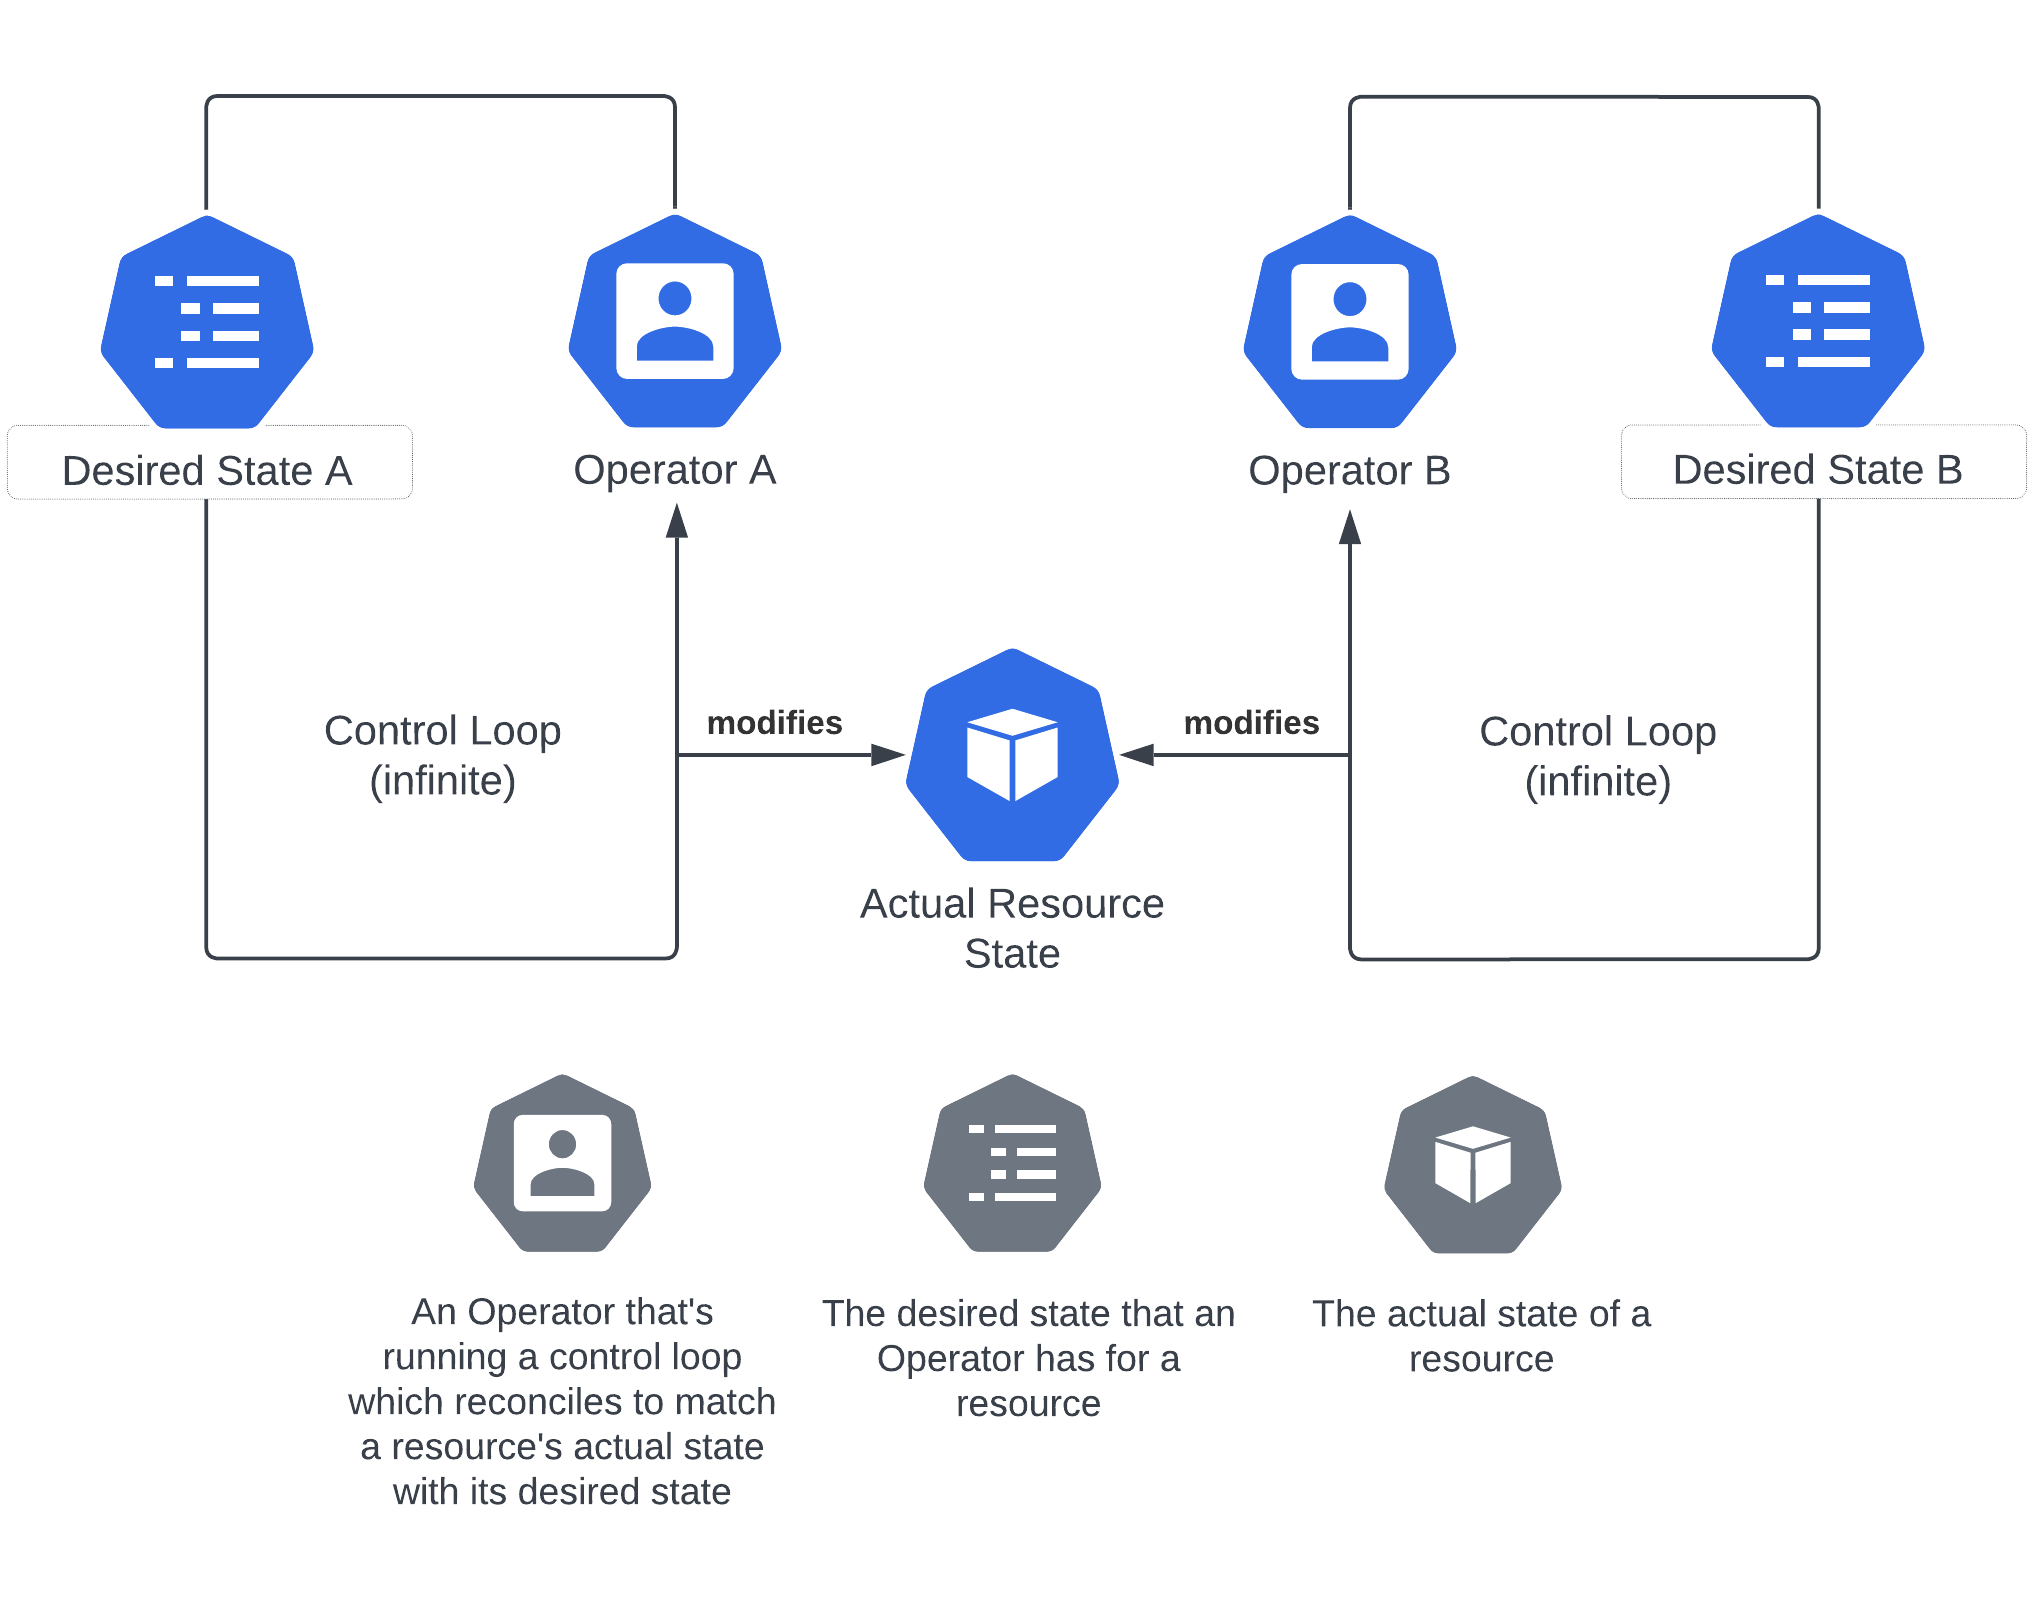
\includegraphics[width=150mm]{new-problem-model.png}
    \caption{Model of The Problem - Two Operators Fighting Over a Resource's State}
    \label{problem-model}
\end{figure}

This pattern works well until two Operators with conflicting desired states are both set to reconcile a resource. This will cause the resource's state to continuously change as both Operators attempt to synchronise its actual state with their unique desired state. The model shown in \hyperlink{problem-model}{Figure \ref{problem-model}} shows this problem in action. Each Operator will do the following:
\begin{enumerate}
    \itemsep0em 
    \item Watch a resource's actual state.
    \item Check the desired state for that resource.
    \item Compare the actual state with the desired state and
    \subitem 3.1. \emph{If they match} then return to Step 1. and repeat.
    \subitem 3.2. \emph{If they don't match} then continue to Step 4.
    \item Modify the resource's actual state so that it matches the desired state.
    \item Repeat this process continuously.
\end{enumerate}



\subsubsection{Industry Example}
As an example, the open-source e-learning platform Moodle can be used. In an education environment, one might have a Moodle Operator and a MySQL Operator to serve as Moodle's database. The MySQL Operator manages the storing, of course, student, and module information. This application may then install a Tutors Operator, which is another e-learning platform which houses course notes and lab work. Since there is already a MySQL database via the MySQL Operator, Tutors can use the same database to store course notes and lab work. 

\begin{figure}[H]
    \hypertarget{moodle-tutors}
    \centering
    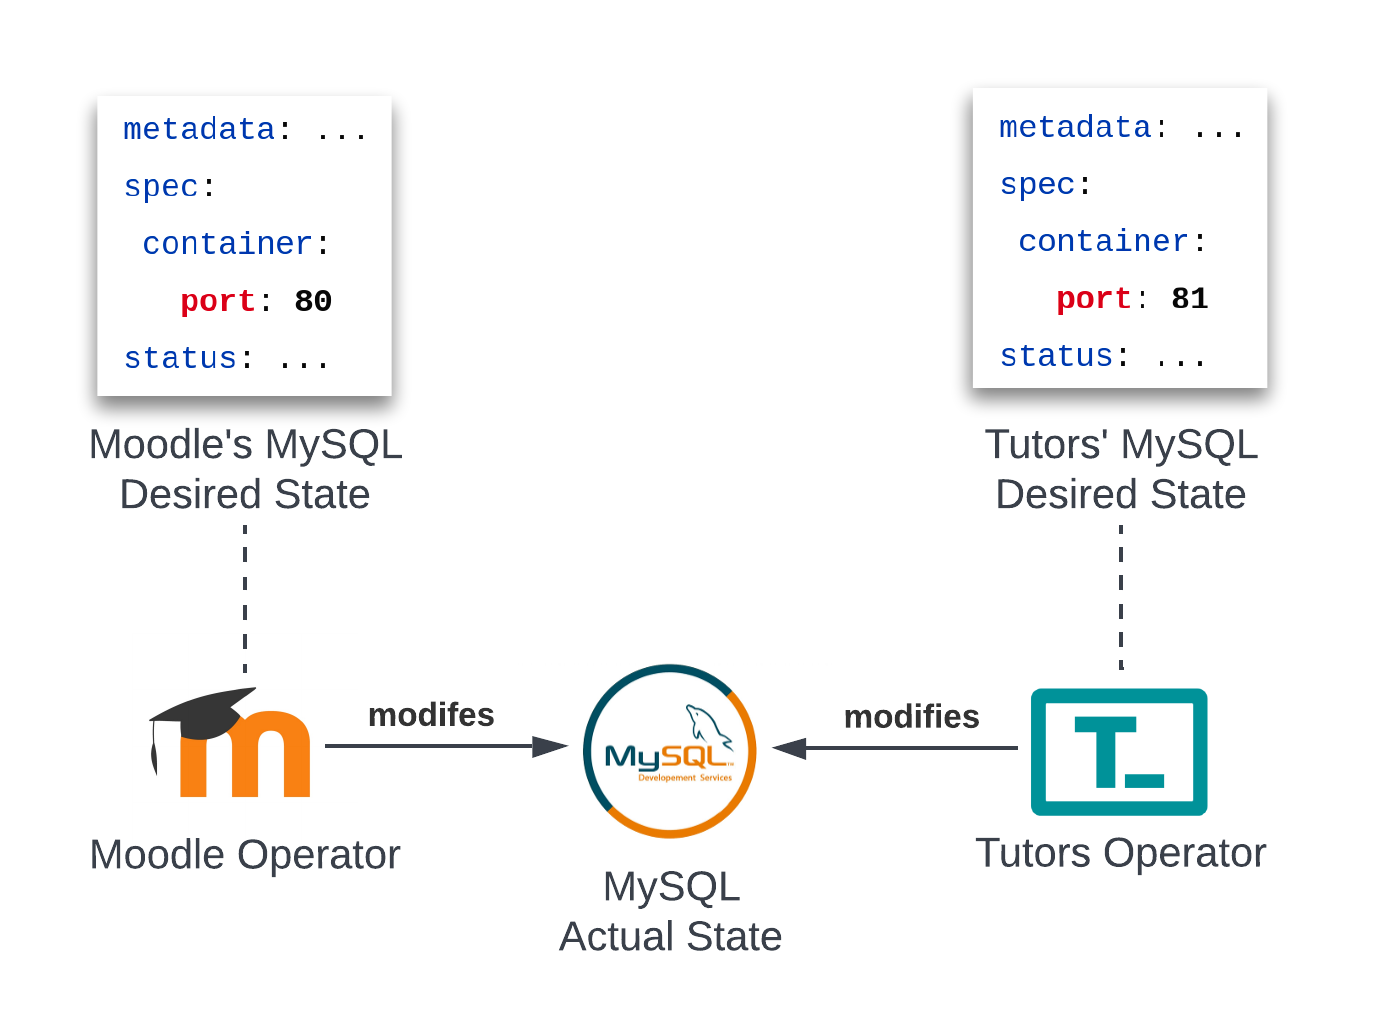
\includegraphics[width=125mm]{new-moodle-example.png}
    \caption{Simplified Model of Moodle, Tutors, and MySQL Industry Example}
    \label{moodle-tutors}
\end{figure}

In this example, it would be very easy to misconfigure one of the Operators to have a dissimilar desired state for the MySQL resource. This would cause both Operators to constantly change that resource. Imagine Moodle wanted the port in which database access occurred to be port 80 and Tutors wanted the database access to occur through port 81. This would cause the MySQL resource's access port to be changed back and forth. If a lecturer or student attempts to access information through Moodle, but at that point in time the MySQL resource's port was configured by the Tutors Operator, the user would not be able to retrieve the data. 

\subsection{Aims and Objectives}
The solution is to create a custom Kubernetes controller which will monitor resource states. A Kubernetes Operator can create a resource, become its owner, and will set the controller to watch that resource for changes. If another operator changes the resource the controller will trigger an alert, notify the developer via a slack integration and allow the developer to fix the problem without the need for time-consuming debugging. 

\begin{figure}[H]
    \hypertarget{solution-model}
    \centering
    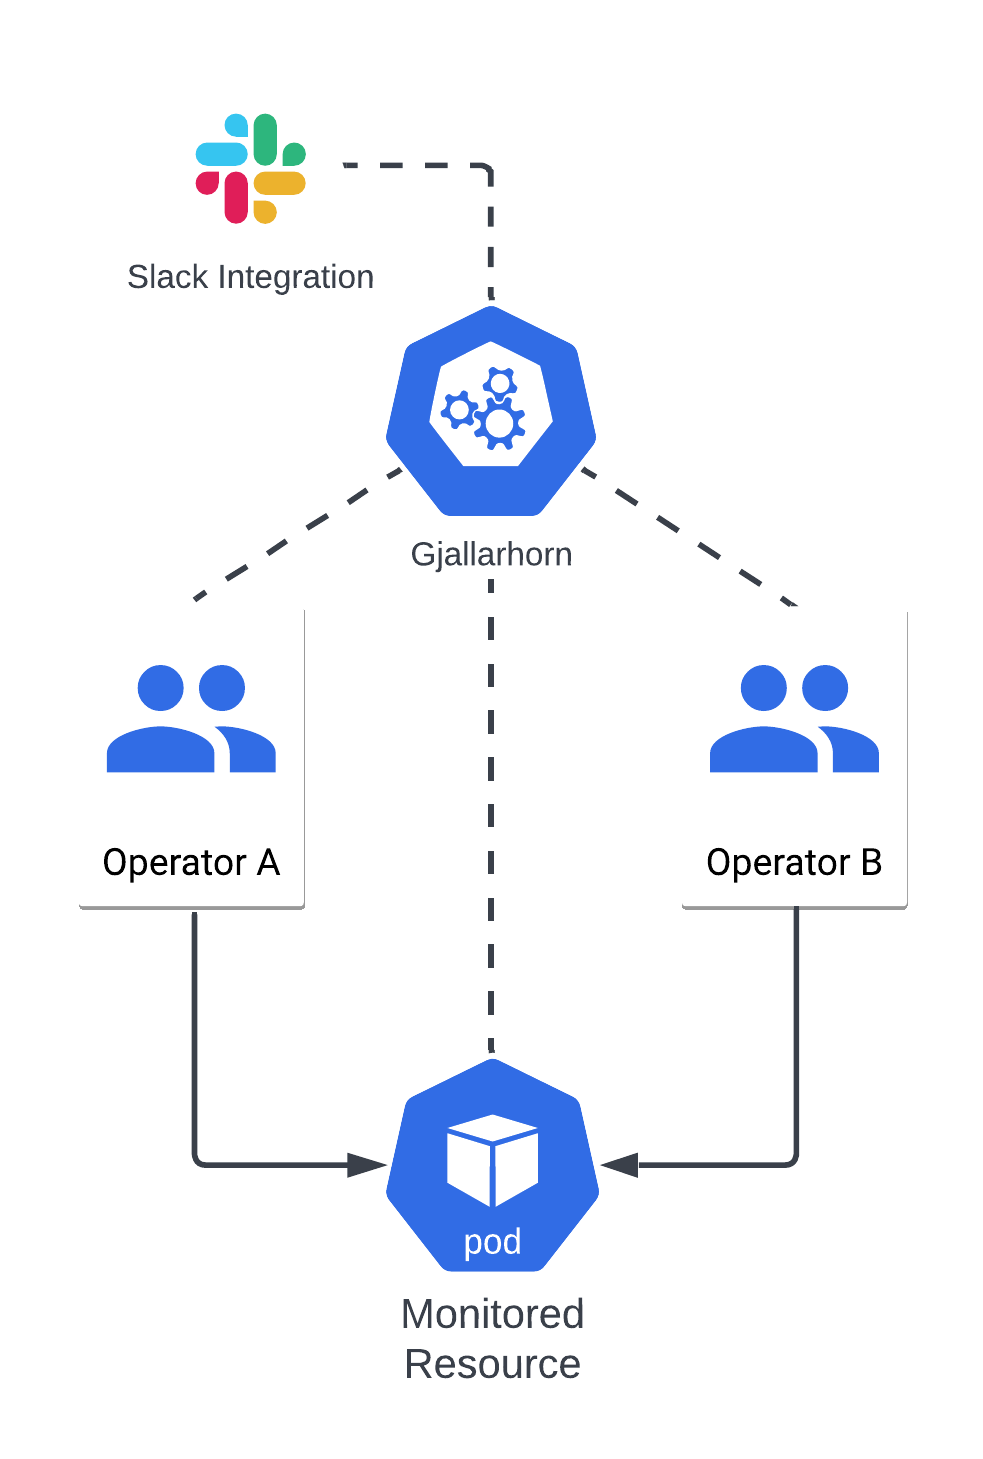
\includegraphics[width=100mm]{solution-model.png}
    \caption{Model of the solution: Heimdall}
    \label{solution-model}
\end{figure}

\hyperlink{solution-model}{Figure \ref{solution-model}} models the proposed solution where the Owner Operator and Rogue Operator are attempting to change a resource's actual state. Once the Owner Operator is installed, it creates the resource with the addition of a label that Heimdall is looking for. Heimdall sees a new resource has been created with this label and begins monitoring its state. The Rogue Operator is installed and begins changing the resource. \\\par The minimum viable product for Heimdall involves the controller watching for non-owners changing the state of a resource. It will then generate an interactive notification for slack with details on the issue to allow the developers to find and fix the problem with relative ease. The stretch goals for Heimdall will involve allowing for an atomic owner of a resource to be set and blocking of changes from non-owners. This will not only allow the developer to fix the problem with ease but also stop the issue from occurring and prevent any downtime for the end user.



\subsection{Risks}
TODO(): this is a risky project as it has never been done before 



\subsection{Contributions}



\subsection{Outline}



\section{Methodology}
The chosen methodology for software development teams is paramount for the successful planning and development of a product. Historically, the Waterfall Methodology was commonplace - but now Agile is the gold standard. Waterfall involved a distinct sequence of actions for engineers to follow. In short, it involved extensive design and planning before ever writing a line of code. Long documents detailing product design and strategy were written to fit the stakeholder's requirements. This proved to be ineffective as in most cases, holes in the design are discovered after beginning the implementation. In recent years, Agile has begun replacing this framework as it has proven much more efficient for software development teams \cite{agile-waterfall}.



\subsection{Agile}
"Agile is an iterative approach to project management and software development that helps teams deliver value to their customers faster and with fewer headaches" \cite{what-is-agile}. TODO()
DISCUSS AGILE + SCRUM



\subsection{Scrum Roles}
Scrum has three main roles: Scrum Master, the Product Owner, and the Development Team. These are used to help describe the responsibilities of each stakeholder for a product.



\subsection{Scrum Artifacts}
Teams who practice Agile and Scrum methodologies often collect Scrum Artifacts. These are pieces of information that a product's stakeholders and the team developing it use to describe its development. The main Scrum Artifacts used for this project include Product Backlog Refinement, Sprint Planning, and Sprint Reviews. There are also various Extended Artifacts that are not included in the official Scrum Artifacts definition. These include reporting mechanisms like Burn down Charts.



\subsection{Version Control}
What is VCS, Git, GitHub, 



\subsection{Continuous Integration}
Version control lies at the heart of Continuous Integration. CI is an Agile practice of integrating code changes to a product automatically from various contributors (product teams and open-source community contributions). It is a method used to consistently merge code changes into one central repository which runs automated tests and builds to ensure code functionality and integrity.   



\subsection{Continuous Delivery}
Continuous Delivery is an approach 



\subsection{Testing Approach}



\subsection{Open Source}



\section{Technologies} \label{technologies} \hypertarget{technologies}{}


\subsection{Kubernetes}



\section{Tools}
Minikube, Kubebuilder, Docker, Podman, Git, GitHub, Jira



\section{Design}



\subsection{System Architecture Overview}



\subsection{Requirements}



\subsection{Functional Requirements}



\subsection{Non Functional Requirements}



\subsection{Core Requirements and Stretch Goals}



\subsection{User Stories}
As a Developer, I want to be aware of changes to resources that I own.
In order to be aware of changes to resources that I own, as a k8s developer, I want to be notified by some channel, such that I don’t have to manually watch resources in a cluster.
As a Developer, I want to control the cadence of alerts so that I can control noise created from alerts.
As a Developer, I want to claim ownership of the resources that I control
As a Developer, I want to control the changes to resources that I own.



\subsection{Personal Stories}
As a student, I want to have achieved First Class Honors, so that I can reach my academic goals
As an aspiring Software Engineer, I want to have contributed a solution to a common problem faced by Software Engineers working with Kubernetes, so that I can make a valuable contribution..?? - something like that



\subsection{User Definitions}



\subsection{Models}



\section{Prototypes}



\subsection{Proof of Concept}



\section{Reflection}



\section{Summary}



\subsection{Review}



\subsection{Semester 2 Outline}



\section{Appendices}



\bibliographystyle{alpha}


\clearpage
\begin{thebibliography}{9}


\bibitem[What is Agile?, 2022]{what-is-agile}
\emph{Atlassian}, \\URL: https://www.atlassian.com/agile 

\bibitem[Operator Pattern, 2022]{operator-pattern}
\emph{Kubernetes}, \\URL: https://kubernetes.io/docs/concepts/extend-kubernetes/operator/

\bibitem[IBM API-Connect, 2022]{understanding-apis}
\emph{Understanding rate limits for APIs and Plans}, \\URL: https://www.ibm.com/docs/en/api-connect/10.0.1.x?topic=connect-understanding-rate-limits-apis-plans

\bibitem[M. McCormick, 2012]{agile-waterfall}
\emph{Waterfall vs Agile Methodology}, M. McCormick, \\2nd ed. MPCS, Inc., 2012.

\bibitem[I. Sommerville, 2021]{agile-book}
\emph{Engineering Software Products: An Introduction to Modern Software Engineering}, 2021.
  
\bibitem[Kubernetes Overview, 2022]{k8s-overview}
\emph{Kubernetes}, \\URL: https://kubernetes.io/docs/concepts/overview/  
\bibitem[Red Hat Developer, 2020]{rhoam-overview}
\emph{Red Hat OpenShift API Management}, Red Hat, Dec. 16, 2020. 
\\URL: https://developers.redhat.com/products/red-hat-openshift-api-management/overview
  


\end{thebibliography}




\end{document}